\documentclass[a4paper]{article}
\usepackage[utf8]{inputenc}

\usepackage{amsthm}
\usepackage{amssymb}
\usepackage{amsmath}
\usepackage{mathtools}

\usepackage[ruled,vlined]{algorithm2e} 
% \usepackage{algorithm}
% \usepackage{algorithmic}
\usepackage{array}
\usepackage{listings}
\usepackage{multirow}
\usepackage{cite}
        
\usepackage[dvipsnames]{xcolor}
\usepackage[toc,page]{appendix}
\usepackage{tikz}
\usepackage{float}
\usepackage{graphicx}
\usepackage{caption} 
\usepackage{subcaption}
\usepackage[colorlinks = true, 
            linkcolor = blue,
            urlcolor  = blue, 
            citecolor = blue,
            anchorcolor = blue]{hyperref}
        
\graphicspath{ {images/} }
\usepackage[a4paper,width=165mm,top=22mm,bottom=22mm]{geometry}
\setlength{\headheight}{15pt}
% \usepackage[most]{tcolorbox}
        
\title{Developing CNN and RNN Models for Time Series Classification with application to ECG Signal Classification}
\author{Ali Khudiyev}
\date{November 2021}

\begin{document}
\maketitle

\begin{abstract}
	Time series classification becomes one of the most important tasks for variety of problems, such as scene analysis, natural language processing, detection of brain diseases, signature verification 
	and so on. Such classification tasks require a deep learning (DL) model to work with sequences of data that are very helpful all together for predictions. This concern of this paper is to 
	distinguish different ECG signals by classifiying them as either normal or abnormal. For this task, CNN and RNN models are developed, tested and evaluated in terms of better accuracy, precision, 
	recall and f1-score. Architectural desing choices and different optimization techniques are discussed throughout the developement of both models and several experimental results are provided with 
	tables and plots for better visualization. Finally, several conclusions have been made according to the statistical data from the carried experiments.
\end{abstract}

\section{Time Series Data}
The given time series dataset is ECG200 from the UCR archive which contains recorded electrical activities during one heartbeat. Each series represent either normal heartbeat or a myocardial infarction. 
A signal consists of 96 points and corresponds to one of two possible outputs - negative($-1$) or positive($1$). Typical ECG signals from the training dataset are as shown below:

\begin{figure}[h]
	\centering
	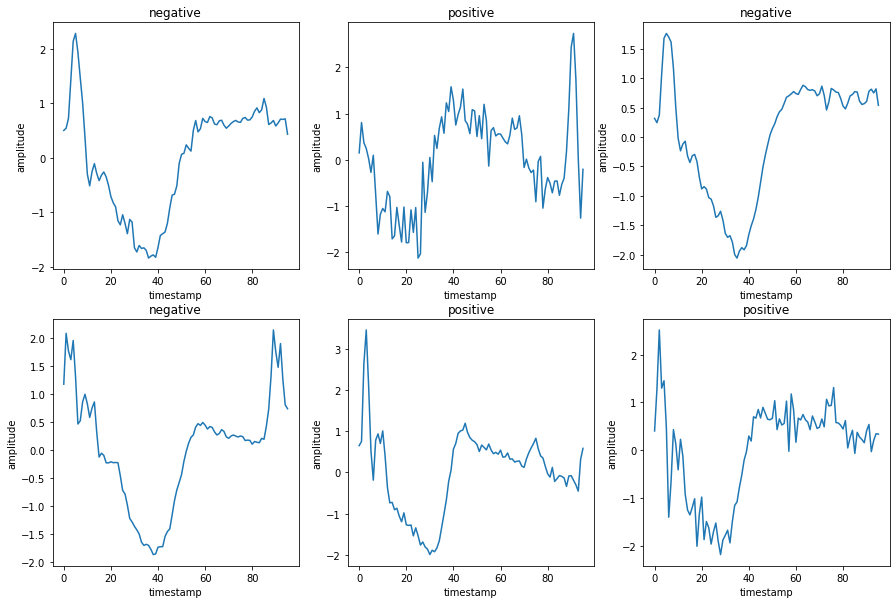
\includegraphics[width=0.8\textwidth]{img/ecg_signals.png}
	\caption{ECG signals}
	\label{fig:signals}
\end{figure}

The data is imbalanced due to the different number of negative and positive samples in both training and testing datasets. In the training dataset, there are 31- and 69+ samples while in the testing dataset,
there are 36- and 64+ samples. There are 100 samples for training and 100 more for testing in total, and the ratio of negative/positive samples within a dataset is preserved with small difference.

\section{Development}
Since there are two possible classes, it is a binary classification task and the inputs have temporal relationship in a sense that each of them is followed by the next one. Convolutional Neural Networks 
(CNNs) and Recurrent Neural Networks (RNNs) are suitable for such classification tasks since kernels and hidden states may help to exploit temporality respectively. These DL models are developed with 
several optimization techniques by using \textit{Keras} from \textit{Tensorflow} library in Python3.

\subsection{Building CNN}
Convolutional Neural Networks (CNNs) have been widely used for many tasks, such as time series prediction, object recognition and so on. Their domain is not necessarily restricted to 2D data since 1D 
or 3D convolutions are also possible to perform. These models take their magic powers from the convolution operator($*$) which is a well-defined operation used to find the nature of modifications made on 
a function by another function in mathematics. CNNs use convolution operator between the input data and kernel(s) to extract important features which can be sent to the fully connected network for prediction.

\begin{figure}[h]
	\centering
	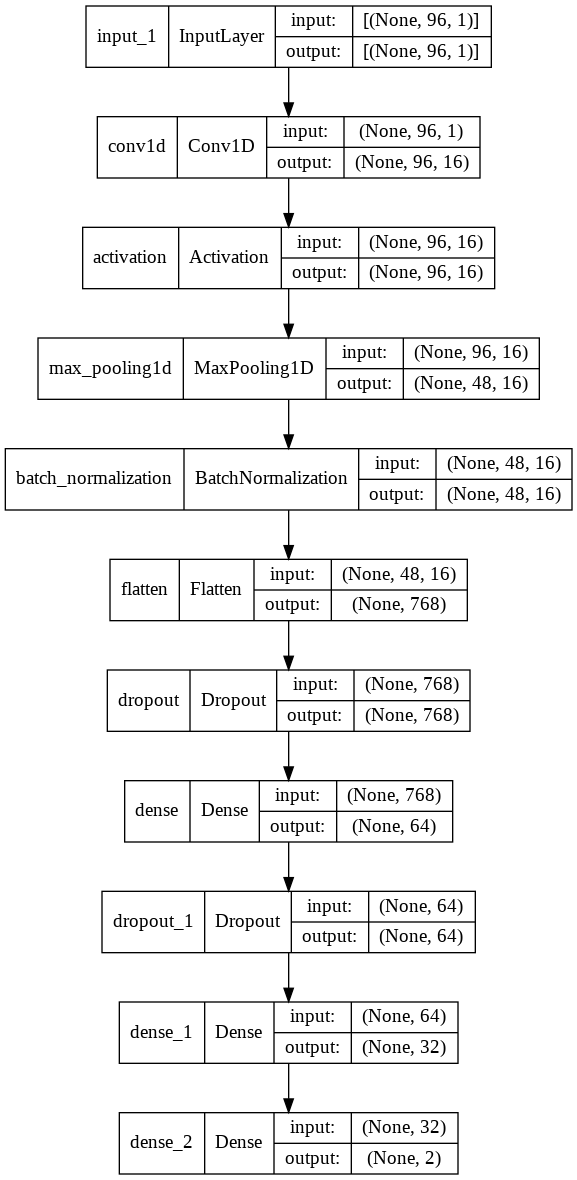
\includegraphics[height=0.8\textwidth]{img/cnn_arch.png}
	\caption{CNN Architecture}
	\label{fig:cnn_arch}
\end{figure}

The figure \ref{fig:cnn_arch} illustrates the architecture of the developed CNN model. Input layer expects the data with the shape of $(96, 1)$ which is connected to a convolutional layer with 16 kernels of 
size of 3 and padding set to \textit{same}. Maxpooling layer follows the convolution layer with size of 2 and is followed by a batch normalization layer. The reason that the batch normalization is put after 
the activation layer is due to the recommendation of several resources \cite{batchAfterActivation1,batchAfterActivation2} which claim that it generally yields better results although the original 
paper \cite{batchnorm} recommended the opposite arhictecture(activation followed by batch normalization). Flattened outputs of the batch normalization layer are connected to a dense layer of 64 units with 
sigmoid activation function and 20\% dropout rate. Another dense layer of 32 units with the same activation function follows and finally, the output layer is a dense layer with 2 units and softmax activation. 
The model is compiled with \textit{Adam} optimizer and \textit{binary crossentropy} loss function and it is trained with the batch size of 64, 300 epochs and 30\% validation split.

Number of convolutional layers and dense layers have found to be somewhat optimal when 1 convolution layer and 2 dense layers are used with the parameters shown above. Some CNN filters are shown in the 
figure \ref{fig:cnn_filters} to illustrate the learned kernel weights. It is obvious from the figures shown below that the convolutional layer extract information mostly based on 2 different ECG values 
(either consecutive or separated by another value) according to the kernels with single black color, and sometimes based on single value according to the kernels with the single white color.

\begin{figure}[h]
	\centering
	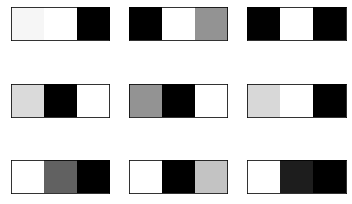
\includegraphics[width=0.5\textwidth]{img/cnn_filters.png}
	\caption{CNN filters}
	\label{fig:cnn_filters}
\end{figure}

Some feature maps that are outputs of the convolution layer are shown in the figure \ref{fig:cnn_feature_maps} and we can see which parts of the ECG signals are main interest areas for the developed CNN model. 
For example, almost all the feature maps start with gray followed by white which is then followed by black color and the positions of these colors are almost the same for each feature map. This means that 
decisions of the model for the patient is highly dependent on the smaller white parts then moderately on gray parts, however, sections with the black color almost has not affect on the outputs.

\begin{figure}[h]
	\centering
	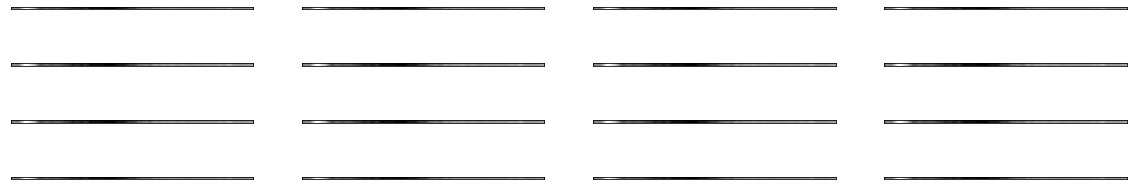
\includegraphics[width=0.75\textwidth]{img/cnn_feature_maps.png}
	\caption{CNN feature maps}
	\label{fig:cnn_feature_maps}
\end{figure}

By looking at the figures shown above, we can say that the model has learned to classify normal and abnormal signals highly based on the first timestamps. If features maps are compared with the original signals, 
the intervals can been observed in a more detailed way.

\subsection{Building RNN}
Recurrent Neural Networks (RNNs) have been widely used for tasks requring time series analysis and unlike CNNs, they do not use convolution operator but instead, they consists of one or more hidden states 
that are helpful to keep track of important information which is necessary for final predictions. There are vanilla RNNs which usually faces with the vanishing gradient problem as the architecture gets 
deeper. The vanishing gradient problem is due to lack of control on the hidden states and it is significantly prevented in the architecture called \textbf{long short-term memory (LSTM)} with the help of 
extra gates known as \textit{forget}, \textit{input} and \textit{output} gates. For this reason, an LSTM layer is used to build a recurrent neural network for the goal of this project.

\begin{figure}[h]
	\centering
	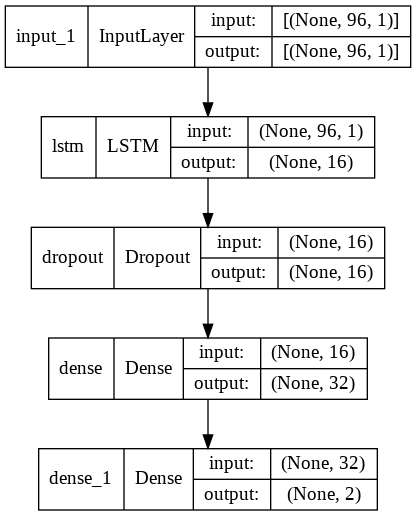
\includegraphics[height=0.4\textwidth]{img/rnn_arch.png}
	\caption{RNN Architecture}
	\label{fig:rnn_arch}
\end{figure}

The figure \ref{fig:rnn_arch} illustrates the developed RNN architecture which consists of relatively less layers than that of the CNN model. The model expects an input of the form $(96, 1)$ which is 
passed to an LSTM layer with 16 hidden states, hyperbolic tangent($\tanh$) as the activation and sigmoid as the recurrent activation function. Then follows a droput layer with 20\% rate connecting to 
another dense layer with 32 units and sigmoid as the activation function. Finally, the last dense layer is added with 2 units and softmax activation function for the output. The model is compiled with 
\textit{Adam} optimizer and \textit{binary crossentropy} loss function and it is trained with the batch size of 64, 300 epochs and 30\% validation split.

When several LSTM layers are added to the model, my experiments showed that it tends to give unstable or worse results. Adding a bunch of dense layers after the LSTM layer(s) did not fix the problem 
either and the experiments showed that the deeper architecture is, more training epochs are required and since there are 100 training samples to train on, increasing the number of epochs causes overfitting 
as it can be clearly observed from the icreasing validation loss after several hundred iterations. Batch size is also set to 64 due to emprical reasons, moreover, when the batch size is less than 64, 
the model tend to give noise loss values and since it is recommend to have a batch size of 2's powers 64 is the maximum batch size less than the number of training samples which is 100.

\section{Experiments}
The experiments have been carried in a classic \textit{Google Colab} environment and each model with the same training parameters have been trained 5 times for benchmarking purposes. The trained CNN model 
has 1 convolutional and 2 hidden dense layers and RNN model has 1 LSTM and 1 hidden dense layer. Overall, the number of trainable parameters is 51458 for CNN and 1762 for RNN. Batch size has been set to 
64 with 300 epochs and 30\% validation split for both models. Formulas for the used metrics to evaluate the model performance is shown below:

\begin{align*}
	\text{Accuracy} &= \frac{\text{TP}+\text{TN}}{\text{TP}+\text{FP}+\text{TN}+\text{FN}} \\
	\text{Precision} &= \frac{\text{TP}}{\text{TP}+\text{FP}} \\
	\text{Recall} &= \frac{\text{TP}}{\text{TP}+\text{FN}} \\
	\text{F1-score} &= 2\cdot\frac{\text{Recall}\cdot\text{Precision}}{\text{Recall}+\text{Precision}}
\end{align*}

\subsection{CNN}
Loss and accuracy metrics for both training(with blue color) and validation(with orange color) sets are shown in the figure \ref{fig:cnn_plot}. It is observed that the current CNN architecture with 100 
training samples tends to overfit when the $\#\text{epochs} > 200$ due to increasing loss and it works just fine when trained in between 150 and 200 epochs. Although accuracy is plotted as the other metrics, 
it is not the only importantant one to measure performance of the models and we can also observe from the graph that the accuracy starts fluctuating after about 130 epochs.

\begin{figure}[h]
	\centering
	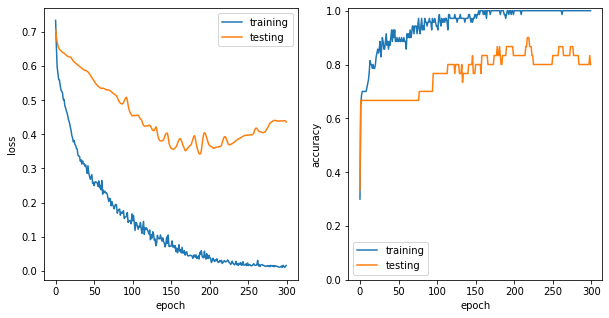
\includegraphics[width=0.8\textwidth]{img/cnn_result.png}
	\caption{Training history of CNN}
	\label{fig:cnn_plot}
\end{figure}

The confusion matrix shown in figure \ref{fig:cnn_prfs} illustrates the TP(True Positives), FP(False Positives), FN(False Negatives) and TN(True Negatives) which are necessary to calculate metrics such as 
accuracy, precision, recall and f1-score. Each row of the matrix represents true labels of the signals whereas each column represents the predicted labels and the numbers that are not in the diagonal(as in 
identity matrix) represents different types of misclassifications.

\begin{figure}[h]
	\centering
	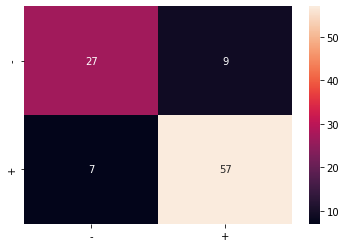
\includegraphics[width=0.5\textwidth]{img/cnn_prfs.png}
	\caption{Confusion matrix}
	\label{fig:cnn_prfs}
\end{figure}

The table shown below is another representation for the confusion matrix which shows the percentage values of each important metric. From the experiments, negative samples have less precision, 
recall and f1-score than that of the positive samples. Support values also indicate that the dataset contains less or exactly 36 negative samples and more or exactly 64 positive samples.

\begin{table}[h]
	\centering
	\begin{tabular}{|c|c|c|c|c|c|c|}
		\hline
		\textbf{Class} & \textbf{Accuracy} & \textbf{Precision} & \textbf{Recall} & \textbf{F1-score} & \textbf{Loss} & \textbf{Support} \\
		\hline
		- & 0.84 & 0.79 & 0.75 & 0.77 & 0.507 & 36 \\
		+ & 0.84 & 0.86 & 0.89 & 0.88 & 0.507 & 64 \\
		\hline
	\end{tabular}
	\caption{CNN Statistics}
	\label{tab:cnn_stats}
\end{table}

\subsection{RNN}
With the same training parameters, RNN gives relatively noisier loss values than that of CNN. After 200 epochs, fluctuations of the loss values are observed for both training and validation. The validation 
loss values start to get into equilibrium whereas training loss tends to decrease which is a warning for potential overfitting.

\begin{figure}[h]
	\centering
	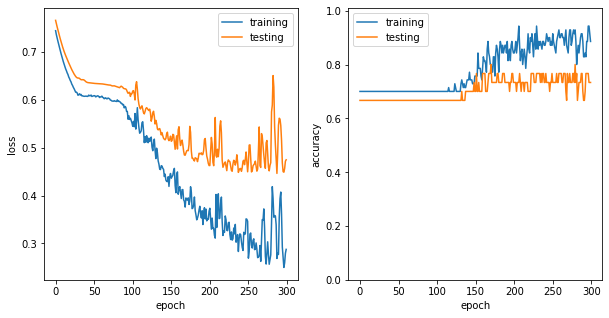
\includegraphics[width=0.8\textwidth]{img/rnn_result.png}
	\caption{Training history of RNN}
	\label{fig:rnn_plot}
\end{figure}

Confusion matrix shows relative poor results than the CNN model due to higher number of misclassification which can be observed from the figure \ref{fig:rnn_prfs} that there are 14 FN and 12 FP in total.

\begin{figure}[h]
	\centering
	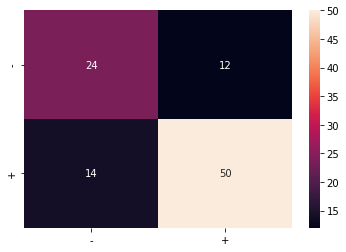
\includegraphics[width=0.5\textwidth]{img/rnn_prfs.png}
	\caption{Confusion matrix}
	\label{fig:rnn_prfs}
\end{figure}

As expected due to the low support value of negative samples, precisison, recall and f1-score metrics show superior results for the positive samples.

\begin{table}[h]
	\centering
	\begin{tabular}{|c|c|c|c|c|c|c|}
		\hline
		\textbf{Class} & \textbf{Accuracy} & \textbf{Precision} & \textbf{Recall} & \textbf{F1-score} & \textbf{Loss} & \textbf{Support} \\
		\hline
		- & 0.74 & 0.63 & 0.67 & 0.65 & 0.506 & 36 \\
		+ & 0.74 & 0.81 & 0.78 & 0.79 & 0.506 & 64 \\
		\hline
	\end{tabular}
	\caption{RNN Statistics}
	\label{tab:rnn_stats}
\end{table}

\section{Results \& Conclusion}
Experiments carried for the both models show that they are almost equally performant in terms of mean loss, accuracy, precision, recall and f1-score values. However, the best accuracy/precision/recall/f1-score 
has been observed with the CNN model. Although both architectures are relatively simple, they are not dramatically bad in terms of the above mentioned metrics. The run-time performance of the developed RNN 
model is slightly better, however, the number of trainable parameters is also almost 30x less than the CNN model. As the table \ref{tab:comparison} illustrates the differences, I can conclude that RNN tends to 
work slower in general which is highly due to the learning process of LSTM layers. Since both models give lower precision for negative samples, it means that patients labeled as negatives have 66-67\% of 
probability to really diagnosed as negative whereas this probability is in between 79-80\% for the ones labeled as positives. Recall or sensitivity values show that if a person is a truely negative sample then 
he/she has 61-63\% probability to be labeled correctly and if a person is a truely positive sample then the probability is in between 82-83\%. Finally, F1-score shows us that the both models almost as good as 
the other with slight differences.

\begin{table}[h]
	\centering
	\begin{tabular}{|c|c|c|}
		\hline
		\textbf{Metrics} & \textbf{CNN} & \textbf{RNN} \\
		\hline
		\textbf{Mean Loss} & 0.527 & 0.52 \\
		\hline
		\textbf{Std Loss} & 0.012 & 0.012 \\
		\hline
		\textbf{Accuracy} & 0.748 & 0.75 \\
		\hline
		\textbf{Precision} & 0.66 | 0.8 & 0.67 | 0.79 \\
		\hline
		\textbf{Recall} & 0.63 | 0.82 & 0.61 | 0.83 \\
		\hline
		\textbf{F1-score} & 0.64 | 0.8 & 0.63 | 0.81 \\
		\hline
		\textbf{Time elapsed(s)} & 42.64 & 40.53 \\
		\hline
	\end{tabular}
	\caption{Comparison between the proposed CNN and RNN models}
	\label{tab:comparison}
\end{table}

\newpage
\begin{thebibliography}{9}
% \bibitem{lamport94}
% Leslie Lamport (1994) \emph{\LaTeX: a document preparation system}, Addison
% Wesley, Massachusetts, 2nd ed.
\bibitem{batchAfterActivation1}
Intro to Optimization in Deep Learning. \url{https://blog.paperspace.com/busting-the-myths-about-batch-normalization/}
\bibitem{batchAfterActivation2}
Batch normalization in 3 levels of understanding. \url{https://towardsdatascience.com/batch-normalization-in-3-levels-of-understanding-14c2da90a338}

\bibitem{batchnorm}
Sergey Ioffe and Christian Szegedy (2015) \emph{Batch Normalization: Accelerating Deep Network Training by Reducing Internal Covariate Shift}, \url{http://arxiv.org/abs/1502.03167}

% @article{DBLP:journals/corr/IoffeS15,
%   author    = {Sergey Ioffe and
%                Christian Szegedy},
%   title     = {Batch Normalization: Accelerating Deep Network Training by Reducing
%                Internal Covariate Shift},
%   journal   = {CoRR},
%   volume    = {abs/1502.03167},
%   year      = {2015},
%   url       = {http://arxiv.org/abs/1502.03167},
%   eprinttype = {arXiv},
%   eprint    = {1502.03167},
%   timestamp = {Mon, 13 Aug 2018 16:47:06 +0200},
%   biburl    = {https://dblp.org/rec/journals/corr/IoffeS15.bib},
%   bibsource = {dblp computer science bibliography, https://dblp.org}
% }
\end{thebibliography}

\end{document}
